\documentclass[tikz]{standalone}
\usepackage[utf8x]{inputenc}
\usepackage{tikz}
\usetikzlibrary{patterns}
\begin{document}
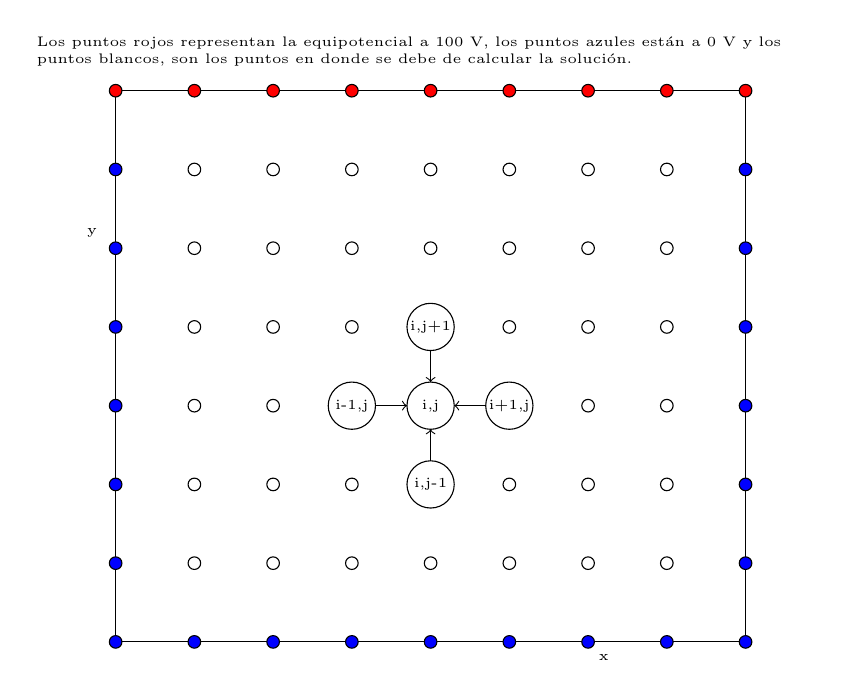
\begin{tikzpicture}[font=\tiny]
	\draw (0, 8) -- (8, 8);
	\draw (0, 1) -- (0, 8);
	\draw (8, 1) -- (8, 8);
	\draw (0, 1) -- (8, 1);
	\draw (6.2, 0.8) node {x};
	\draw (-0.3,6.2) node {y};

	\foreach \x in {0, 1, 2, 3, 4, 5, 6, 7, 8}
		\draw [fill=red](\x, 8) circle (0.08);
	
	\foreach \x in {1, 2, 3, 4, 5, 6, 7}
		\draw [fill=blue](\x, 1) circle (0.08);
	
	\foreach \x in {1, 2, 3, 4, 5, 6, 7}
		\draw [fill=blue](8, \x) circle (0.08);

	\foreach \x in {1, 2, 3, 4, 5, 6, 7}
		\draw [fill=blue] (0, \x) circle (0.08);

	\foreach \x in {1, 2, 3, 4, 5, 6, 7	}
		\foreach \y in {2, 3, 4, 5, 6, 7}
			\draw [fill=white] (\x, \y) circle(0.08);
	
	\draw [fill=white](4,4) circle(0.3);
	\draw [fill=white](3,4) circle(0.3);
	\draw [fill=white](5,4) circle(0.3);
	\draw [fill=white](4,3) circle(0.3);
	\draw [fill=white](4,5) circle(0.3);
	\draw (4,4) node {i,j};
	\draw (3,4) node {i-1,j};
	\draw (5,4) node {i+1,j};
	\draw (4,3) node {i,j-1};
	\draw (4,5) node {i,j+1};
	\draw [arrows=->] (3.3,4) -- (3.7,4);
	\draw [arrows=->] (4.7,4) -- (4.3,4);
	\draw [arrows=->] (4,3.3) -- (4,3.7);
	\draw [arrows=->] (4,4.7) -- (4,4.3);
	\node[text width=10cm] at (4, 8.5) {Los puntos rojos representan la equipotencial a 100 V, los puntos azules están a 0 V y los puntos blancos, son los puntos en donde se debe de calcular la solución.};
\end{tikzpicture}
\end{document}